\documentclass[final]{beamer}

% ====================
% Packages
% ====================
\usepackage{amsfonts}
\usepackage[T1]{fontenc}
\usepackage{lmodern}
\usepackage[size=custom,width=30,height=48,scale=1.0]{beamerposter}
\geometry{paperwidth=30in,paperheight=48in}
\usetheme{gemini}
\usecolortheme{ucf}
\usepackage{graphicx}
\usepackage{booktabs}
\usepackage{tikz}
\usepackage{pgfplots}
\pgfplotsset{compat=1.17}
\usepackage{xcolor}  % For custom colors

% ====================
% Custom color for header
% ====================
\definecolor{customgreen}{HTML}{20ff6a}  
\setbeamercolor{headline}{bg=customgreen}  % Apply custom green to header

% ====================
% Block title colors
% ====================
\setbeamercolor{block title}{fg=black,bg=customgreen}  % All regular blocks green
\setbeamercolor{block title alerted}{fg=black,bg=yellow}  % Alert blocks stay yellow
\setbeamercolor{block title example}{fg=black,bg=blue}    % Example blocks (if any)
% ====================
% Lengths
% ====================
\newlength{\sepwidth}
\newlength{\colwidth}
\setlength{\sepwidth}{0.025\paperwidth}
\setlength{\colwidth}{0.3\paperwidth} % Adjust column width if needed

\newcommand{\separatorcolumn}{\begin{column}{\sepwidth}\end{column}}

% ====================
% Title
% ====================
% ====================
% Title
% ====================
\title{\LARGE Intelligent Traffic Management System using \\[0.2em]
       \Large CNN-YOLOv7 with Integrated MQTT Protocol}
       
\author{\normalsize Mann Manohar, Sai Chandra Mouli, Mithilesh Walde}

\institute[Indian Institute Of Information Technology, Nagpur]{
  \normalsize Indian Institute Of Information Technology, Nagpur \\ 
  \small \textit{Computer Vision \& IoT Project}
}

% ====================
% Footer (optional)
% ====================
\footercontent{
  \href{https://iiitn.ac.in}{https://iiitn.ac.in} \hfill
  Intelligent Traffic Management \hfill
  \href{mailto:bt22eci017@iiitn.ac.in}{bt22eci017@iiitn.ac.in}
  |
  \href{mailto:bt22eci035@iiitn.ac.in}{bt22eci035@iiitn.ac.in}
  |
  \href{mailto:bt22eci056@iiitn.ac.in}{bt22eci056@iiitn.ac.in}}

% Ensure the bottom is not forced to stretch
\raggedbottom

% ====================
% Document Start
% ====================
\begin{document}

% Add the new header color change in the document
\addtobeamertemplate{headline}{}
{
    \begin{tikzpicture}[remember picture,overlay]
      \node [anchor=north west, inner sep=3cm] at ([xshift=0.0cm,yshift=2.5cm]current page.north west)
      {
\includegraphics[height=9cm]{logoss/image.png}}; % also try shield-white.eps
      \node [anchor=north east, inner sep=3cm] at ([xshift=1.0cm,yshift=2cm]current page.north east);
    \end{tikzpicture}
}

% ====================
% Frame Content
% ====================
\begin{frame}[t]
\begin{columns}[t]

% ====================
% Column 1
% ====================
\begin{column}{\colwidth}

  \begin{block}{Abstract}
    
    Urban traffic congestion is a growing problem, leading to increased travel times, fuel consumption, and pollution. Traditional traffic management systems often rely on predefined schedules or simple loop detectors, lacking adaptability to real-time conditions. This poster presents an Intelligent Traffic Management System (ITMS) leveraging state-of-the-art computer vision techniques, specifically Convolutional Neural Networks (CNNs) and the YOLOv7 object detection model. The system analyzes real-time video feeds to detect and classify vehicles, pedestrians, and potentially other relevant objects. This information is used to estimate traffic density and flow. The Message Queuing Telemetry Transport (MQTT) protocol is integrated for efficient, lightweight communication between sensing nodes (cameras with processing units) and a central control system or other infrastructure components, enabling dynamic traffic signal adjustment and data dissemination.
  \end{block}

  \begin{block}{Introduction}
    
    Effective traffic management is crucial for modern cities. Conventional systems struggle with dynamic traffic variations, leading to inefficiencies. Computer vision offers a powerful alternative by enabling direct observation and analysis of traffic scenes.
    \begin{itemize}
      \item \textbf{Challenge:} Static signal timings and limited sensing capabilities of traditional systems.
      \item \textbf{Solution Approach:} Utilize Deep Learning, specifically CNNs and YOLOv7, for accurate, real-time object detection from traffic cameras.
      \item \textbf{Communication:} Employ MQTT for scalable and low-latency data exchange in a distributed system architecture.
      \item \textbf{Goal:} Develop an adaptive ITMS capable of optimizing traffic flow, enhancing safety, and providing real-time traffic insights.
    \end{itemize}
    This system aims to replace or augment existing infrastructure with intelligent, vision-based monitoring and control.
  \end{block}

  \begin{block}{Core Technologies}

    
    \textbf{1. Convolutional Neural Networks (CNNs)} \par
    CNNs are a class of deep neural networks highly effective for image analysis tasks. They use convolutional layers to automatically learn hierarchical spatial features from input images, making them ideal for object recognition.
    \begin{itemize}
      \item Architecture: Composed of convolutional, pooling, and fully connected layers.
      \item Function: Feature extraction (edges, textures, shapes, objects).
      \item Application: Forms the basis for many object detection models, including YOLO.
    \end{itemize}


    \textbf{2. YOLOv7 (You Only Look Once)} \par
    YOLOv7 is a state-of-the-art, real-time object detection algorithm. It processes entire images at once, predicting bounding boxes and class probabilities simultaneously.
    \begin{itemize}
      \item Type: Single-stage detector.
      \item Strengths: High speed (suitable for real-time video) and competitive accuracy. Architecture includesoptimizations for efficiency and performance.
      \item Output: Bounding box coordinates (x, y, width, height), confidence score, and class label (e.g., car, truck, pedestrian, traffic light) for each detected object.
      \item Use Case: Detecting and classifying vehicles/pedestrians in traffic video streams.
    \end{itemize}


    \textbf{3. MQTT (Message Queuing Telemetry Transport)} \par
    MQTT is a lightweight, publish/subscribe messaging protocol designed for constrained devices and low-bandwidth, high-latency networks. Ideal for IoT and distributed systems.
    \begin{itemize}
      \item Paradigm: Publish/Subscribe. Decouples message producers (publishers) from consumers (subscribers).
      \item Broker: A central server manages message distribution based on topics.
      \item Benefits: Low network overhead, scalability, asynchronous communication.
      \item Role in ITMS: Transmitting detected object counts, traffic density metrics, or control signals between cameras, processing units, and traffic controllers.
    \end{itemize}
  \end{block}

  \vfill

  \begin{alertblock}{Important Point}
    \centering
    \textbf{Scan QR code for more details}
    \begin{figure}[h]
        \centering
        
\includegraphics[width = 0.3\textwidth]{logoss/dipqr.png}
        \label{fig:my_zero}
    \end{figure}
  \end{alertblock}







\end{column}

\separatorcolumn

% ====================
% Column 2
% ====================
\begin{column}{\colwidth}

  \begin{block}{System Architecture \& Methodology}

    \textbf{1. Video Acquisition:} Cameras capture real-time video streams from traffic intersections or road segments.

    \textbf{2. Preprocessing (Optional):} Frames may undergo preprocessing steps like resizing or normalization for optimal input to the detection model.

    \textbf{3. Object Detection (YOLOv7):}
    \begin{itemize}
      \item Each frame is fed into a pre-trained or fine-tuned YOLOv7 model.
      \item The model outputs bounding boxes, class labels (car, bus, person, etc.), and confidence scores for all detected objects.
    \end{itemize}

    \textbf{4. Data Extraction \& Analysis:}
    \begin{itemize}
      \item Information from YOLOv7's output is processed to:
          \begin{itemize}
            \item Count vehicles/pedestrians per lane or region of interest.
            \item Estimate traffic density or queue lengths.
            \item Detect specific events (e.g., accidents, jaywalking - requires further logic).
          \end{itemize}
      \item This data forms the basis for traffic management decisions.
    \end{itemize}

    \textbf{5. MQTT Communication:}
    \begin{itemize}
      \item The processing unit publishes extracted data (e.g., vehicle counts) to specific MQTT topics (e.g., `traffic/junction1/lane2/count`).
      \item Subscribers (e.g., traffic light controllers, central monitoring dashboard) receive relevant data from the MQTT broker.
      \item Example Topic Structure: `sensor location/data type` 
    \end{itemize}

    \textbf{6. Control \& Actuation / Monitoring:}
    \begin{itemize}
      \item Based on subscribed MQTT data, traffic light controllers can dynamically adjust signal timings.
      \item Data can be visualized on dashboards for monitoring purposes.
      \item Alerts can be generated for incidents.
    \end{itemize}

    \textbf{YOLOv7 Model Details:}
    \begin{itemize}
      \item Typically uses models pre-trained on large datasets like COCO.
      \item Can be fine-tuned on specific traffic datasets for improved accuracy in target environments.
      \item Requires sufficient computational resources (GPU recommended for real-time performance).
    \end{itemize}
  \end{block}

  \begin{block}{Visual Demonstration \& Results}
    
    The system's core capability is demonstrated through processing sample traffic video frames.
    
    \begin{figure}[h!]
      \centering
      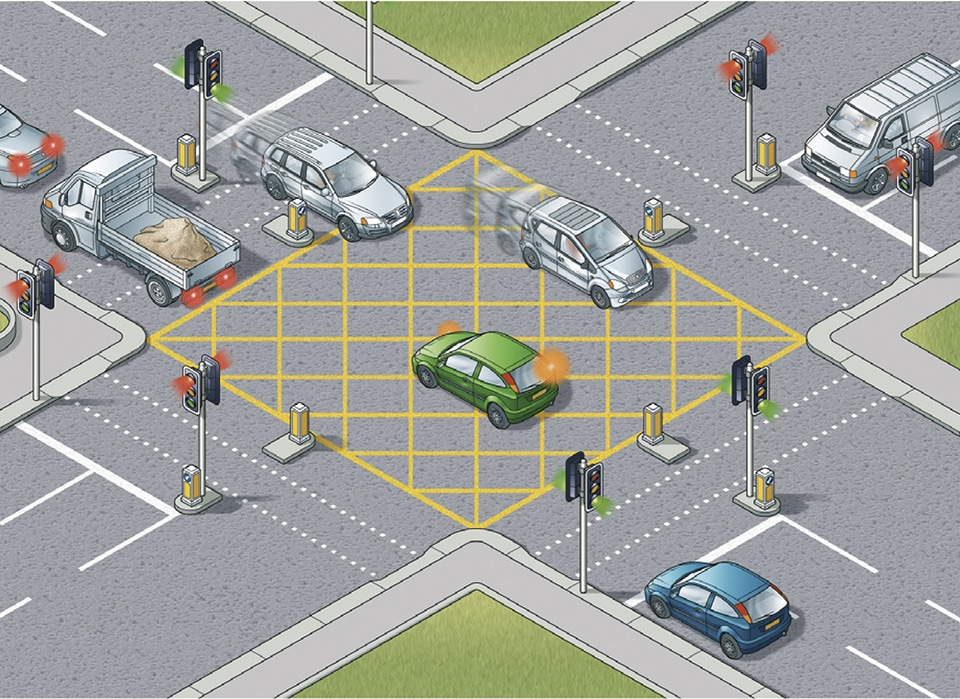
\includegraphics[width=0.8\linewidth]{rule-174-enter-a-box-junction-only-if-your-exit-road-is-clear_orig.jpg}
      \caption{ Original Traffic Scene Frame}
      \label{fig:original-traffic}
    \end{figure}
    \begin{figure}[h!]
      \centering
      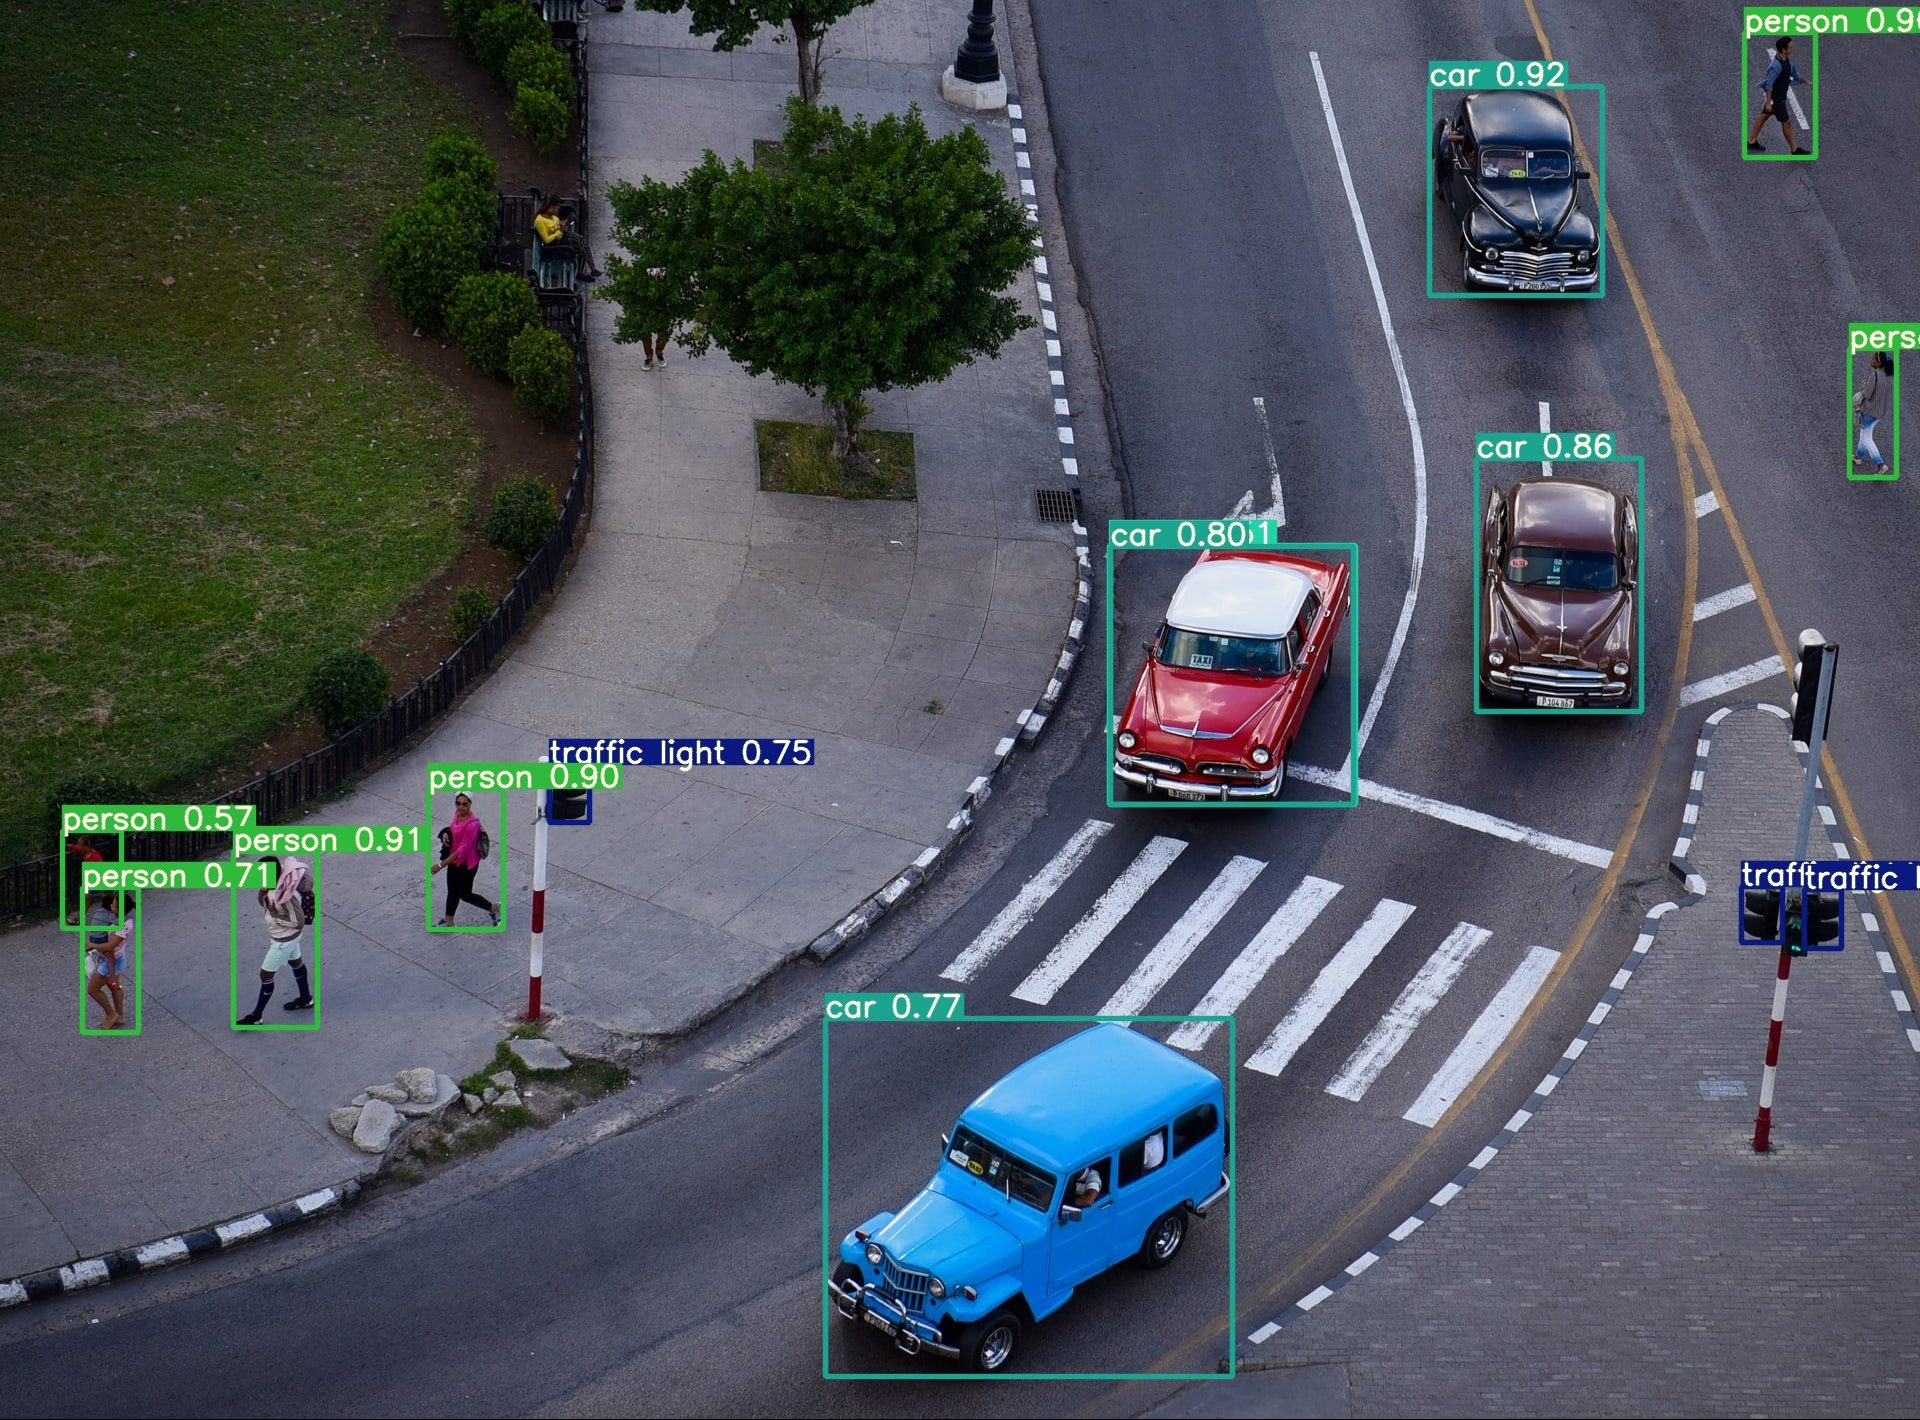
\includegraphics[width=0.8\linewidth]{jeremy-stewardson-yolov7-e1657792694411.jpg}
      \caption{ YOLOv7 Classification Results}
      \label{fig:yolo-classification}
    \end{figure}
  \textbf{Observations:}
    \begin{itemize}
      \item YOLOv7 accurately detects various vehicles and pedestrians even in moderately complex scenes.
      \item Detection speed allows for real-time processing on suitable hardware.
      \item Extracted counts and locations provide valuable data for traffic analysis.
      \item MQTT enables flexible communication for integrating diverse system components.
    \end{itemize}
  \end{block}

  \vfill

\end{column}

\separatorcolumn

% ====================
% Column 3
% ====================
\begin{column}{\colwidth}

  \begin{block}{Discussion}
   
    \textbf{Advantages:}
    \begin{itemize}
      \item \textbf{Real-Time Adaptability:} Enables traffic signal control based on actual demand, reducing delays.
      \item \textbf{Rich Data Acquisition:} Provides detailed information (vehicle types, counts, pedestrian presence) beyond simple vehicle detection.
      \item \textbf{Accuracy \& Speed:} YOLOv7 offers a strong balance for real-time traffic object detection.
      \item \textbf{Scalability \& Flexibility:} MQTT allows easy integration of multiple sensors and control units.
      \item \textbf{Non-Intrusive Installation:} Camera-based system avoids road closures needed for installing in-ground sensors.
      \item \textbf{Incident Detection Potential:} Can be extended to detect accidents, stalled vehicles, or traffic violations.
    \end{itemize}

    \textbf{Limitations \& Challenges:}
    \begin{itemize}
      \item \textbf{Computational Cost:} Real-time YOLOv7 processing often requires dedicated GPUs, increasing deployment cost.
      \item \textbf{Environmental Factors:} Performance can be affected by adverse weather (rain, fog, snow), poor lighting (night, glare), and occlusions (large vehicles blocking smaller ones).
      \item \textbf{Camera Requirements:} Needs well-positioned cameras with sufficient resolution and clear lines of sight.
      \item \textbf{Training Data Dependency:} Model performance relies heavily on the quality and diversity of the training dataset.
      \item \textbf{MQTT Broker Reliability:} System availability depends on the MQTT broker's uptime and performance.
      \item \textbf{Privacy Concerns:} Use of cameras for monitoring requires addressing potential privacy issues.
    \end{itemize}

    \textbf{Future Work \& Enhancements:}
    \begin{itemize}
      \item Integrate multi-camera views for wider coverage and handling occlusions.
      \item Incorporate tracking algorithms (e.g., DeepSORT) for trajectory analysis and flow estimation.
      \item Optimize models (e.g., using TensorRT, pruning) for deployment on edge devices.
      \item Develop more sophisticated traffic prediction and control algorithms.
      \item Fuse vision data with other sensor types (e.g., Radar, LiDAR) for enhanced robustness.
      \item Implement security measures for MQTT communication.
    \end{itemize}
  \end{block}

  \begin{block}{Conclusions}
   
    The proposed Intelligent Traffic Management System successfully demonstrates the potential of combining advanced computer vision (CNN/YOLOv7) with efficient IoT communication (MQTT).
    \begin{itemize}
      \item YOLOv7 provides accurate and fast detection of relevant traffic objects.
      \item CNNs form the foundation for powerful visual understanding.
      \item MQTT enables scalable and decoupled communication within the system.
    \end{itemize}
    This approach offers significant advantages over traditional methods by providing richer data and enabling real-time adaptive control strategies. While challenges related to environmental factors and computational requirements exist, the system presents a promising direction for improving urban mobility, reducing congestion, and enhancing road safety. Further development and optimization can lead to robust and widely deployable intelligent transportation solutions.
  \end{block}

  \vfill

\begin{block}{References}
    \begin{thebibliography}{9}
      \bibitem{yolo}
      Wang, C. Y., Bochkovskiy, A., \& Liao, H. Y. M. (2023). \textit{YOLOv7: Trainable bag-of-freebies sets new state-of-the-art for real-time object detectors}. \\
      \url{https://arxiv.org/abs/2207.02696}
      
      \bibitem{cnn}
      LeCun, Y., Bengio, Y., \& Hinton, G. (2015). \textit{Deep learning}. Nature, 521(7553), 436-444. \\
      \url{https://doi.org/10.1038/nature14539}
      
      \bibitem{mqtt}
      MQTT Standard v5.0. (2019). \textit{OASIS Standard}. \\
      \url{https://docs.oasis-open.org/mqtt/mqtt/v5.0/os/mqtt-v5.0-os.html}
      
      \bibitem{dataset}
      Lin, T. Y., et al. (2014). \textit{Microsoft COCO: Common Objects in Context}. \\
      \url{https://arxiv.org/abs/1405.0312}

      \bibitem{edge_computing}
      Shi, W., Cao, J., Zhang, Q., Li, Y., \& Xu, L. (2016). \textit{Edge computing: Vision and challenges}. IEEE Internet of Things Journal, 3(5), 637-646. \\
      \url{https://doi.org/10.1109/JIOT.2016.2579198}
      
      \bibitem{traffic_vision}
      Chen, Z., Ellis, T., \& Velastin, S. A. (2012). \textit{Vehicle detection, tracking and classification in urban traffic}. In 15th International IEEE Conference on Intelligent Transportation Systems (pp. 951-956). \\
      \url{https://doi.org/10.1109/ITSC.2012.6338629}
      
      \bibitem{smart_transport}
      Guo, J. (2021). \textit{Contribution and mechanism of different levels of educational human capital to the identification of regional green economic growth}. Computational Intelligence and Neuroscience, 2021, 34824578. \\
      \url{https://doi.org/10.1155/2021/4105716}
    \end{thebibliography}
\end{block}

\end{column}

\end{columns}
\end{frame}

\end{document}